\subsubsection{Scattering light noise in optical cavities}\label{app:scatter}
%\emph{Author(s): K Kokeyama, H. L\"{u}ck, A. Freise}

\begin{comment}
We have estimated the scattering between suspended mirrors for
different cavities geometries to determine whether this process
affects the selection of the geometry of the  ET filter cavities.

% scattering process
Deviations from a perfect mirror surface can scatter the main laser beam.
Scattered fields propagate along arbitrary spurious paths inside the cavity.
In general,  when the wavefront of the scattered light is changed
by deformations of the mirror surfaces,
the scattering into any direction is given by the Fourier transform of the mirror surface.
The longer spatial wavelengths presented in the mirror surface give smaller scattering angles.
A typical mirror surface has more long spacial wavelengths
than short spacial wavelengths, therefore, the scattering angle will be very small.

The scattered light propagates along spurious paths and reaches the detection port,
it couples to the main beam to create phase noise.
At the same time some scattered light fields may go out of the cavity and are lost.
This contributes to the optical loss, and the amount of the loss depends on the number of mirrors
in the cavity, and the mirror bidirectional distribution function (BRDF).
%
Here, we consider only the phase noise effect for this geometry analysis.

% Three scenarios
For the four cavity geometries, the following three scattering scenarios were considered:
\begin{itemize}
\item Direct back scattering.
When the main beam is reflected by a mirror, a part of the light field is scattered back
by the non-uniform distribution of the mirror surface.
% explain
Considering mirror angles, this effect is expected to be relatively small.
%The scattered field couples with the cavity resonant mode
%in the opposite direction in respect to the propagation direction of the main beam,
%just after being scattered by one mirror.
%%% small angle, large angle, special frequency of the mirror surface
 (triangular, rectangular, and bow-tie cavities)
%
%
\item Diagonal path scattering in a rectangular cavity.
In a rectangular cavity, when the main beam illuminates a mirror,
scattered light is emitted and propagates along the diagonal lines of the rectangular geometry.
After propagating along the diagonal path,
this field goes back into the cavity and reaches at the detection port,
resulting in the phase noise.
%
%
\item Gaussian tail effect.
In the rectangular and bow-tie cavities, the tail of the Gaussian field
may interact with the wrong mirror, for example as shown in Fig.~\ref{fig:Gtail1},
and is partially reflected. This reflected field couples into the main Gaussian beam.
\end{itemize}
\begin{figure}
\centering
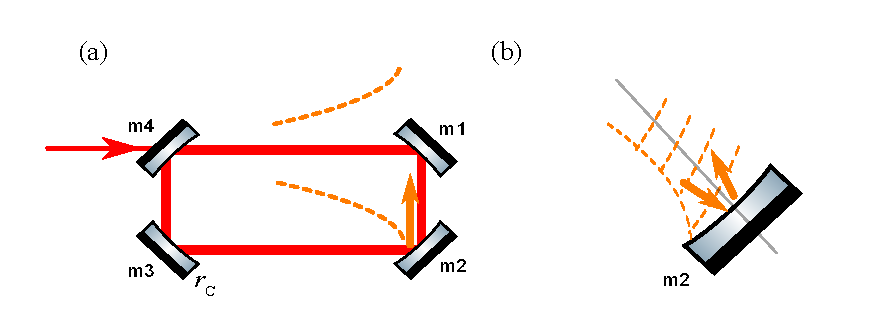
\includegraphics[width=0.7\textwidth]{./Sec_Optics/Gtail.pdf}
\caption{One exemplary path of (a) Direct back scattering.
This occurs at all mirrors except the linear cavity.
(b) Diagonal path scattering. This occurs only in the rectangular geometry.
(c) Gaussian tail effect. The rectangular or bow-tie cavities have this effect.
In addition to the exampled paths shown here, all the possible paths
were considered and summed to evaluate the scattering noise level.}
\label{fig:Gtail1},
\end{figure}

% Coupling factor
The convolution between the scattered field and the main beam was numerically calculated
to evaluate the coupling between the scattered field and the fundamental mode.
As the detailed optical parameters, such as the optimum beam sizes, are not fixed
for filter cavities yet, ET arm cavity parameters were used, e.g.,
the cavity length of 10 km and the mirror radius of 0.31 m.

% result and summary
The direct back scattering was found to be at a negligible scattering level.
This is because the wavefront of the scattered light is changed
when it is reflected by the angled mirror surface in all geometries,
and the wavefronts of the scattered light and the main field do not overlap or couple.
%
Additionally, this scenario is expected to be negligible
also because a typical mirror surface has more long spacial wavelengths
than short spacial wavelength, therefore,
most of the scattering occurs at much smaller angles than in this scenario
(for example the angle is 45 degrees in the rectangular cavity).
As mentioned above, a typical mirror surface has longer spacial wavelength components,
and the scattering angle due to this effect will be very small.

When the closer two long paths are separated by 1 m (between m1 and m2 in Fig~\ref{fig:Gtail1}),
The Gaussian tail effect is found to be negligible, as well.

One has to be careful when considering the scattering field propagating
along the diagonal paths in the rectangular cavity.
In order to block the diagonal paths, placing baffles
inside the rectangular geometry will be useful
to prevent the scattered light propagating along the base paths.

This analysis is also applicable to the ET arm cavities as well as
the filter cavities.
\end{comment}




We have estimated the amount of scattering in long baseline cavities
between the suspended optics for
different cavities geometries to test whether this particular class of scattering
has any influence on the selection of the optical resonator  for ET filter cavities.
The four cavity geometries depicted in Fig.~\ref{fig:new1} were considered.

% new version note
At the detection port, a photodetector detects the light field as
\begin{eqnarray}
P_{\rm out}=E E^*.
\end{eqnarray}
%
In addition to the cavity fundamental mode $E_c$,
we also consider a complex field $\delta E$ which occurs due to scattering,
thus we write
\begin{eqnarray}
E=E _c + \delta E.
\end{eqnarray}
The detected field is proportional to
\begin{eqnarray}
P _{\rm det} &\propto & (E _c + \delta E) (E_c^* +\delta E ^*)\\
&\propto & |E_c| ^2 + |\delta E| ^2 + E_c \delta E ^* + E _c ^* \delta E
\end{eqnarray}
where the first term is the power of the main mode,
and the second term is the power of the scattering filed
which is the second order term and assumed to be negligible.
Only the cross terms between the fundamental and complex scatter field
affects the sensitivity.
%
Considering the x-y plane, the cross term, or coupling factor, is written as
\begin{eqnarray}
\label{eq:couple}
X=\int ^{\infty} _{-\infty} \int ^{\infty} _{-\infty} E _c (x,y,z)
\delta E ^* (x,y,z) {\rm d}x {\rm d}y,
\end{eqnarray}
where
%$E _{\rm sc}(x,y,z_{\rm sc})$ is the scattered light field,
%$z_{\rm sc}$ is the location when the scattering  process occurs
the $z$ axis is the main beam propagation direction,
%and $z _{\rm cav}$ is the locations of the target field coupled by the scattered light.
and $E _{\rm cav}(x,y,z _{\rm cav})$ is the Gaussian field which is the resonant mode in the cavity,
%and the scattered field $\psi _{\rm sc}(x,y,z_{\rm sc})$ coupled into this mode:
\begin{eqnarray}
E _{\rm c}(x,y,z)=\sqrt{\frac{k_0}{\pi z_R}} \frac{i z_R}{z+i z_R}
\exp \biggl[ \frac{-i k_0 (x^2 +y^2)}{2(z+i z_R)} \biggr]
\end{eqnarray}
where $z_R$ is the Rayleigh range of the cavity resonant mode and $k_0$
is the wave number of the laser source.


\begin{figure}
\centering
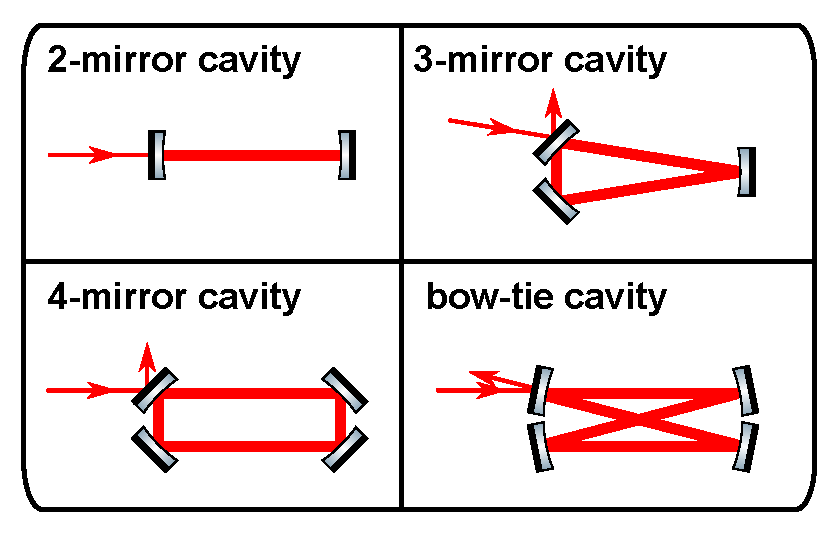
\includegraphics[scale =0.6]{./Sec_Optics/cavity-designs.pdf}
\caption{The scattering-light effects for four geometries,
(1) Two-mirror cavity, (2) triangular cavity, (3) rectangular cavity,
and (4) bow-tie cavity, are analysed.}
\label{fig:new1}
\end{figure}

\begin{figure}
\centering
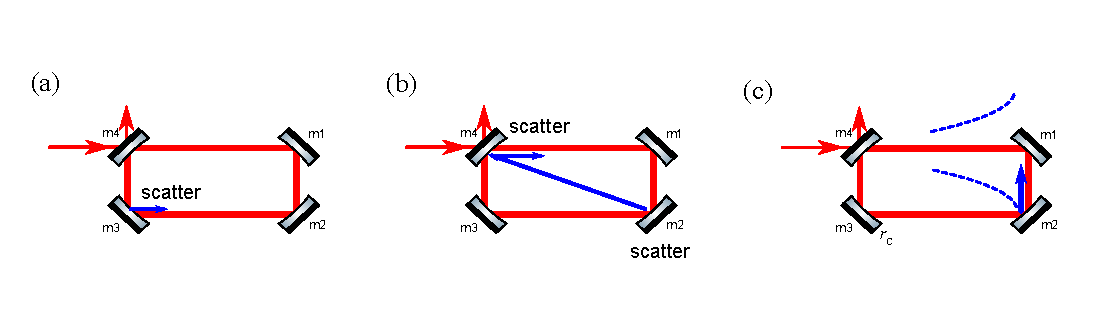
\includegraphics[scale =1]{./Sec_Optics/process.pdf}
\caption{Three scattering processes considered in this analysis.
(a) An exemplary field of the direct back scattering. It occurs at all mirrors
in each geometry except in the two-mirror cavity.
(b) Diagonal path scattering. In the rectangular cavity, the diagonal paths
in the rectangular geometry create spurious paths.
(c) Gaussian tail effect. In the rectangular and bow-tie cavities,
the tail of the Gaussian field may interact
with the wrong mirror, is partially reflected.
This reflected field couples into the main Gaussian beam. }
\label{fig:process}
\end{figure}


% how to evaluate
Here, we consider three simplified scenarios of scattering processes,
in order to estimate the scattered light levels in candidate ET cavities;
direct back scattering, diagonal path scattering,
and the Gaussian tail effect.
The three processes will be evaluated and compared between the four
cavity geometries:
a two-mirror cavity, triangular cavity, rectangular cavity, and bow-tie cavity,
as shown in Fig.~\ref{fig:new1}.

% coupling coefficient
%\subsection{Coupling factor}
%To evaluate the effect of the scattered light noise,
%we calculate how much the scattered field coupling into the cavity mode.
%The coupling factor between the scattered field
%is defined as a convolution between them.
%In other words, the convolution term
%between the scattered fields and the cavity resonant field
%is the cross term when the light field is detected by a photo detector
%because this cross term will appear on the photo detector:
%\begin{eqnarray}
%\label{eq:couple}
%X=\int ^{\infty} _{-\infty} \int ^{\infty} _{-\infty} \psi _{\rm sc} (x,y,z_{\rm sc})
%\psi ^* _{\rm cav}(x,y,z _{\rm cav}) {\rm d}x {\rm d}y,
%\end{eqnarray}

%$\psi _{\rm cav}(x,y,z _{\rm cav})$ propagates in the normal or opposite direction
%$+z$ or $-z$, respectively) depending on the scattered process (see following sections).
%If a lot of the scattered field couples to the cavity mode and resonates in the cavity,
%the scattering loss will cause.




\paragraph{(a) Direct back scattering}
When the main beam is reflected by a mirror, some of the main light field is scattered back
by the non-uniform distribution of the mirror surface.
The scattered field can couple with the cavity resonant mode
in the opposite direction with respect to the propagation direction of the main beam.
The direct back scattering scenario considers only coupling
which occurs after scattering by just one mirror.
%%% small angle, large angle, special frequency of the mirror surface
In general,  when the wavefront of the scattered light is changed
by deformations of the mirror surfaces,
the scattering into any direction is given by the Fourier transform
of the mirror surface figure.
For mirror surface deformations with longer spatial wavelengths
the scattering angle will be smaller.
A typical mirror surface has more long spatial wavelength deformations
than short spatial wavelength deformations,
therefore the power scattered into large angles should be very small.

To evaluate the coupling factor, the scattered field is written as
%
\begin{eqnarray}
\label{eq:direct}
%\begin{split}
%\psi _{\rm sc}(x,y,z) = \psi _{\rm cav}(x,y,-z) \, \exp \bigl[ -2ik_0 M(x,y) \bigr] m(x,y,\alpha)\\
\delta E (x,y,z) = \eta(\phi) E _{\rm c}(x,y,-z) \,
\exp  \Big[ -2ik_0 x \tan \alpha +\frac{i k_0 (x^2+y^2)}{2 r_C} \Bigr],
%\end{split}
\end{eqnarray}
where the exponential factor describes the phase delay due to the mirror angle $\alpha$
with respect to the mirror normal,
and the radius of curvature of the mirror $r_C$
is taken into account as the phase delay due to the reflection surface geometry.

In Eq. (\ref{eq:direct}),
$\eta _n (\phi _{n})$ is an amplitude, or efficiency of the scattering process.
We assumed $\eta$ using the bidirectional reflectance distribution
function (BRDF) which
describes the scattering intensity distribution of a mirror as follows:
The amplitude of the field scattered at angle $\phi _n$ is written as
\begin{eqnarray}
\eta (\phi )&=&\sqrt{P(\phi )}.
\end{eqnarray}
where $P(\phi )$ is the field power that reaches the reflecting mirror surface
at the end of the diagonal path.
The power can be estimated using the BRDF as,
\begin{eqnarray}
P(\phi ) \sim P_0 {\rm BRDF}(\phi ) dS
\end{eqnarray}
where $P_0$ is the incident light power,
$dS$ is the solid angle of the second mirror, which receives the scattered light,
from the first mirror.
As the BRDF of the ET mirrors is unknown,
we use a measured BRDF of an Advanced LIGO mirror~\cite{Yamamoto2011}
\begin{eqnarray}
{\rm BRDF}(\phi )&=&\frac{10^{-20} \pi ^2}{\lambda ^3 \phi {[\rm m^{-3}rad^{-1}]} +0.0016 \lambda \phi ^3 {[\rm m^{-1}rad^{-3}]}}.
\end{eqnarray}
as plotted in Fig. \ref{fig:BRDF}.
Note that this is a BRDF of a silica mirror of Advanced LIGO
and might be an overestimate for the advanced mirrors of ET.
Also, the BRDF is valid when the incoming beam is perpendicular
to the mirror surface, which is different from our situation.
The bidirectional reflectance distribution might alter in our case, in which
the incoming beam and the mirror normal have an angle.

Substituting Eq. (\ref{eq:direct}) into Eq. (\ref{eq:couple}),
we obtain the coupling coefficient as
\begin{eqnarray}
\begin{split}
X_1= \frac{\eta(\phi) k_0 z_R}{\pi (z^2+z_R^2)} \int_{\infty}^{\infty} \int_{\infty}^{\infty}
\exp \Bigl[-\frac{k_0 z_R (x^2 + y^2)} {z^2+z_R^2} \qquad \qquad  \\
-i k_0\bigl\{ \frac{x^2 + y^2}{2 r_C}  %+2 M(x,y)
+2 x \tan\alpha \bigr\} \Bigr] {\rm d}x {\rm d}y.
\end{split}
\end{eqnarray}


\paragraph{(b) Diagonal path scattering}
%The statistical sum

\begin{figure}
\centering
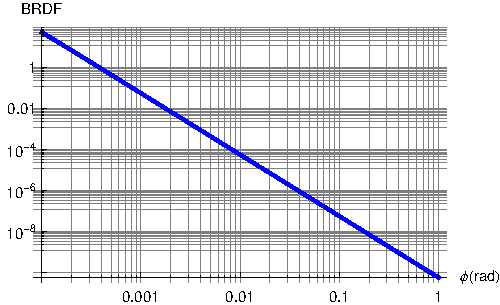
\includegraphics[scale =1]{./Sec_Optics/BRDF-plot.pdf}
\caption{A bidirectional reflectance distribution function (BRDF) of an Advanced LIGO mirror.
The BRDF describes an angular distribution of a scattered light power per
unit solid angle. It was used to assume the scattering efficiency for the
diagonal path scattering process.}
\label{fig:BRDF}
\end{figure}



\begin{figure}
\centering
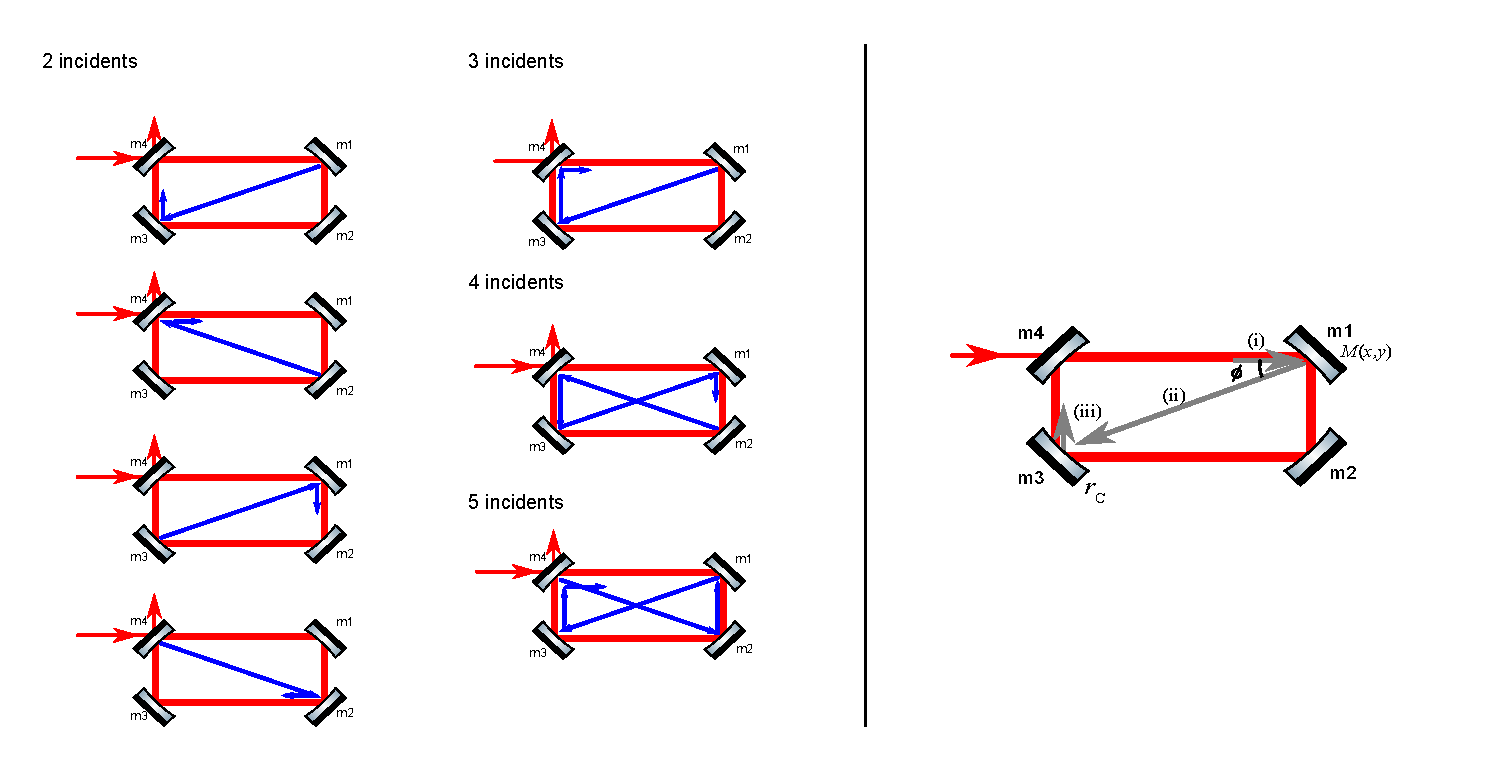
\includegraphics[scale =0.6]{./Sec_Optics/diagonal1.pdf}
\caption{Above left:
Possible routes of the diagonal path scattering.
After the scattered light is emitted by one mirror,
the field propagates along the diagonal path or the shorter path in the rectangular,
then is scattered again or reflected by another mirror,
and finally couples to the main beam. Until coupling into the main beam,
the route is composed of a number of scattering and/or reflection incidents.
Depending on which small angle, large angle scattering, or reflection incident,
one route might have different combinations of spurious paths.
Here, spurious routes with up to 5 incidents were considered.
All possible paths with two incidents are depicted on the left,
while only one example route is shown for 3, 4 and 5 incidents.
Above right:
Example view of small angle scattering and of large angle scattering.
(i)~The scattered light is emitted when the main beam hits m1.
(ii)~The scattered light propagates along the diagonal line.
This incident is considered as the large angle scattering which has a small
scattering efficiency because this diagonal path
is at almost 90 degrees from the main path after the reflection at m1.
(iii)~The scattered field is scattered again at a small angle
with respect to the main beam. This is considered as the small angle scattering
as this path coupling into the main beam is at a very small angle compared with
the reflected path resulting from the diagonal path (from m1).
Depending on whether the scattering angle is large or small,
the corresponding scattering efficiency is taken into account.}
%Upper right panel: scattering process of diagonal path with the large angle
%at the second scattering. Processes~(i) and (ii) are the same as the left panel.
%(iii)~The scattered field is scattered again at a large angle by mirror m3 with its mirror map $M2(x,y)$
%and couples into the Gaussian cavity mode.
%Lower right panel: all the possible incidents of diagonal path II process.
%Similar to the diagonal-I process, $\phi_1$ and $\phi_2$ depend on the paths.
%For example, both $\phi_1$ and $\phi_2$ are small for the gray process,
%on the other hand, $\phi_1$ is large and $\phi_2$ is small for the magenta process.
%The amplitude of the scattered light strongly depends on the scattered angle
%which is summarized in
%Tables~\ref{table:SCcond1} and \ref{table:SCcond2} for all the possible paths.}
\label{fig:diagonal1}
\end{figure}


% path explanation
In the rectangular cavity,
the diagonal lines of the rectangular geometry can become scattered light paths.
When the main beam illuminates a mirror, scattered light fields are produced
by the mirror surface distribution.
The scattered light experiences further scattering or reflection incidents.
There can be many possible spurious paths during this process.
In Fig.~\ref{fig:diagonal1}, all the possible routes with 2 incidents are
shown, while only one example path is shown for other paths
with 3 to 5 incidents. Each route might have one or more spurious paths
because each incident is either from scattering or reflection.
For example, a 3-incident route of m1 - m3 - m4 has
possible paths of m1 (large angle scattering)
- m3 (small-angle and short-path scattering)
- m4 (small angle scattering),
and m1 (large angle scattering) - m3 (reflection)
- m4 (small-angle and short-path scattering),
and m1 (large angle scattering) - m2 (small-angle and short-path scattering)
- m3 (reflection).
Here, we consider such spurious paths with up to 5 incidents.

% counting condition
The total number of possible paths were counted in the following way:
(i) Spurious paths with up to 5 incidents of scatter and/or reflection were considered.
(ii) At the end of the path, the scattered field couples into the main beam in the normal propagating direction. (iii) Direct back scatter was not considered because it is assumed to be smaller than
the coupling in the normal direction at the small angle
(iv) scattered light does not propagate along the long path without coupling into
the main beam.
The total number of the possible spurious paths are
4 paths (all of which are shown in the Fig. \ref{fig:diagonal1}), 10 paths,
12 paths, and 16 paths were found for 3, 4, and 5 incidents, respectively.
To obtain the result, all contributions from all paths are statistically summed.

% small scattering, large scattering, small close scattering
The efficiency of the scattering power is large when the scattering angle,
which is the angle made with the main beam path, is small,
and the efficiency is small when the scattering angle is large.
Therefore, the amplitude of the scattered field depends on the propagation path
and the spurious path.
Here we assume the amplitude using BRDF
which is a function of the scattering angle again.

%After the light field is scattered by the first mirror and propagate the diagonal path,
%there are two possibility to be scattered again at the second mirror.
%The diagonally propagating field is scattered again with small or large scattering angle or large angle,
%as depicted in the left or right panel of Fig.~\ref{fig:diagonal1}, respectively.
%As the incident at a small scattering angle has larger scattering efficiency compared
%with one at the large scattering angle because the most field is scattered to a small angle
%due to the longer spacial frequency of a typical mirror surface, as mentioned above.
%In total, eight paths are considered here.
%For each path, the scattered angles and the coupling direction
%are summarized in Tables~\ref{table:SCcond1} and \ref{table:SCcond2}.

Assuming the scattered field to be a plane wave as a rough approximation,
one can write the scattered field of each path as
\begin{eqnarray}
\label{eq:D1}
%\psi _{\rm sc}(x,y,z) =\frac{\eta (\phi _1) \eta (\phi _2)}{R _d}
%~\exp \Bigl[-i k_0 R_d -2ik_0 M(x,y) +\frac{i k_0 (x^2 +y^2)}{2 r_C} \Bigr]
\begin{split}
\label{eq:D2}
\delta E(x,y,z) =\prod _{n=1}^{N} \eta_n (\phi _n)
\, \exp \Bigl[-i k_0 \bigl\{ R_d +\frac{x^2 +y^2}{2 r_C} \bigr\} \Bigr].
\end{split}
\end{eqnarray}
where $R_d$ is the total path length from the emission point
to the coupling point,
and $r_C$ is the radius of curvature of a mirror when the scattered filed
couples into the cavity, %$M(x,y)$ is the mirror surface map
%of the mirror where the scattered light occurs.
$N$ is the total incidence number,
and $\eta _n (\phi _{n})$ is the amplitude (or efficiency) of the $n$th
incident of scattering or reflection, assumed by BRDF and
the scattering angles.


Substituting Eq.~(\ref{eq:D1}) into Eq.~(\ref{eq:couple}),
the coupling coefficient is derived as
\begin{eqnarray}
%\begin{split}
%X_2= \sqrt{\frac{z_R k_0}{\pi}} \frac{\eta (\phi)}{R_d (z_R +i z_{\rm cav})}
%\int_{\infty}^{\infty} \int_{\infty}^{\infty}
 %\exp \Bigl[-i k_0\bigl\{ R_d+\frac{x^2+y^2}{2 r_C} \qquad \\
%-\frac{x^2+y^2}{(z_{\rm  cav}-i z_R)}+M(x,y)
%\bigr\} \Bigr] {\rm d}x {\rm d}y.
%\end{split}
\begin{split}
X_2= \sqrt{\frac{k_0 z_R}{\pi}} \frac{\prod _{n=1} ^N \eta _n (\phi _n)}{ (z_R +i z _{\rm cav})}
\int_{\infty}^{\infty} \int_{\infty}^{\infty}
\exp \Bigl[-i k_0\bigl\{ R_d+\frac{x^2+y^2}{2 r_C} \qquad \\
-\frac{x^2+y^2}{2(z _{\rm cav}-i z_R)}%+M_1(x,y)+M_2(x,y)
\bigr\} \Bigr] {\rm d}x {\rm d}y.
\end{split}
\end{eqnarray}




%\subsection{Diagonal path scattering II}
%In the rectangular cavity, another coupling process by the diagonal path should be taken into account.
%Similarly to the previous process, the scattered light from one mirror propagate the diagonal path
%as a spherical wave as in the process considered in the previous section.
%Again, spherical waves are possibly overestimate for the propagation,
%but used as a rough approximation.
%Then the scattered field is scattered again by the second mirror
%and couples into the Gaussian cavity mode (upper right panel of Fig.~\ref{fig:diagonal1}).
%As shown in the lower right panel of Fig.~\ref{fig:diagonal1},
%there are four processes possible in a rectangular cavity.

%The light filed after the second scattering is written as
%\begin{eqnarray}
%\begin{split}
%\label{eq:D2}
%\psi _{\rm sc}(x,y,z) =\frac{\eta (\phi _1) \eta (\phi _2)}{R _d}
%~\exp \Bigl[-i k_0 \bigl\{ R_d +\frac{x^2 +y^2}{2 r_C} \\
%+M_1(x,y) +M_2 (x,y) \bigr\} \Bigr].
%\end{split}
%\end{eqnarray}
%where $\phi _1$ is the angle between the main beam and the diagonal path
%when the first scattering, and $\phi _2$ are the angles between the diagonal path
%and the cavity path when the scattered field couples again into the cavity mode.
%%Depending on which path it takes,  $\phi _1$ and  $\phi _2$ are defferent

%Substituting Eq.~(\ref{eq:D2}) into Eq.~(\ref{eq:couple}),
%the coupling coefficient is derived as
%\begin{eqnarray}
%\begin{split}
%X_3= \sqrt{\frac{k_0 z_R}{\pi}} \frac{\eta (\phi _1) \eta (\phi _2)}{R_d (z_R +i z _{\rm cav})}
%\int_{\infty}^{\infty} \int_{\infty}^{\infty}
%\exp \Bigl[-i k_0\bigl\{ R_d+\frac{x^2+y^2}{2 r_C} \qquad \\
%-\frac{x^2+y^2}{2(z _{\rm cav}-i z_R)}+M_1(x,y)+M_2(x,y)
%\bigr\} \Bigr] {\rm d}x {\rm d}y.
%\end{split}
%\end{eqnarray}



\paragraph{(c) Gaussian tail effect}
In the rectangular and bow-tie cavities, the tail of the Gaussian field
may reach the wrong mirror, for example as shown in Fig.~\ref{fig:Gtail} (a),
and is partially reflected. This reflected field couples into the main Gaussian beam.
Note that this is also a simplified picture.
As shown in Fig.~\ref{fig:Gtail} (b), the wave front at the edge of the main field
faces a different direction compared with the wave front at the center
of the beam, therefore, the reflection angle may differ from the main beam path.
However, for a simple estimation, we approximate that
the Gaussian tail field is reflected and directly couples into the main mode.
The rectangular or bow-tie cavity has four fields to be considered
since this process can occur at each mirror.

When a mirror (therefore the coupling point) is a distance $L$ away in the $x$ direction
from the main beam, the coupling field is written as
\begin{eqnarray}
\delta E (x,y,z) =E _c  (x+L _s,y,z _{\rm sc}).
\end{eqnarray}

The coupling coefficient is
\begin{eqnarray}
\begin{split}
X_4=\frac{-k_0 z_R}{\pi (i z _{\rm cav}+z_R) (iz _{\rm sc}-z_R)}\qquad \qquad \qquad \qquad \qquad \qquad \\
\int_{\infty}^{\infty} \int_{\infty}^{\infty}
\exp \Bigl[-i k_0 \Bigl\{
\frac{x^2+y^2}{2(i z_R-z _{\rm cav})}+\frac{(L_s+x)^2+y^2}{2(i z_R-z _{\rm sc})} \Bigr\}
\Bigl]  {\rm d}x {\rm d}y.
\end{split}
\end{eqnarray}


\begin{figure}
\centering
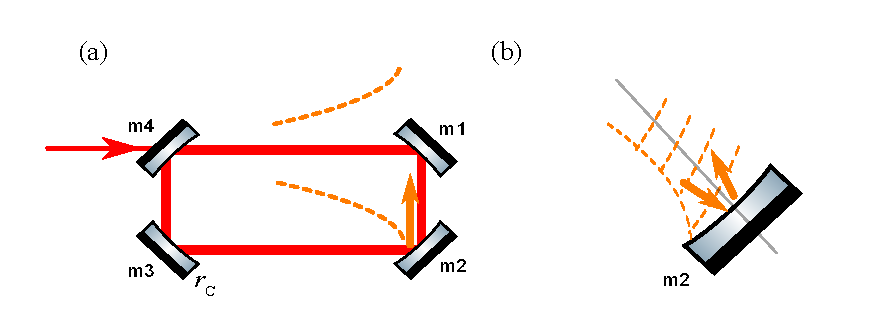
\includegraphics[scale =1]{./Sec_Optics/Gtail.pdf}
\caption{(a) An example dagram of the Gaussian tail effect. This process will occur at each mirror
in the rectangular and bow-tie cavities.
(b) Detailed diagram of the wave fronts at the tail of Gaussian field.
In the picture, the incident angle and the reflection angle
is slightly different from the approximated picture (a).}
\label{fig:Gtail}
\end{figure}


\paragraph{Numerical evaluation}

In order to numerically calculate the coupling coefficient,
we assume that the round trip of a cavity is about 10 km,
and the waist position of the laser beam is at the middle point of the round trip
for all the geometries, as shown in Fig.~\ref{fig:geo-summary}.
The triangular cavity is an isosceles triangle with two 5 km arms and with a 1 m base,
and the beam waist is at the middle of the short path.
The rectangular cavity has long and short paths of 5 km and 1 m respectively,
and the beam waist is at m2 in Fig.~\ref{fig:geo-summary}.
The bow-tie cavity has four paths of 2.5 km
and the separation between the closer mirrors is assumed to be 1 m.
For mode-matching, each mirror was assumed to be either flat
or to have a radius of curvature $r_C$.
%ET fake mirror maps simulated using a sum of
%Zernike polynomials with maximum 1 nm amplitude were used \cite{bond10}.


\begin{figure}
\centering
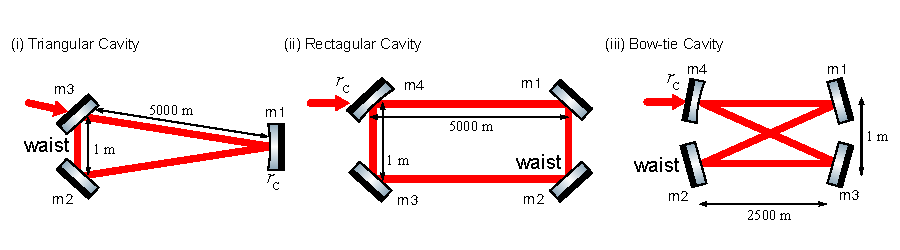
\includegraphics[scale =1]{./Sec_Optics/geo-summary.pdf}
\caption{Cavity designs used for the numerical calculation.
The cavities have a round trip length of approximately
10 km, and a beam waist at the middle point of the path.}
\label{fig:geo-summary}
\end{figure}


$\bullet$  Direct back scattering:
Fig.~\ref{fig:scat-plot-1} shows the plot of $X_1$ over the mirror angle $\alpha$
for four coupling locations ($z$=1, 1000, 2500, {\rm and} 5000).
$X_1$ strongly depends on the angle between
the mirror normal and the propagation direction of the beam, $\alpha$.
The coupling coefficient rapidly approaches zero
when the angle is larger than $10^{-3}$ degrees.
This is because the coupling between the two fields is
very small when the wavefront of one field is delayed
by the mirror surface with the incident angle while the other field is not delayed.
Since the mirror angles of all the ring cavities have much larger $\alpha$,
the direct back-scattering is negligible in ET cavities
although arbitrary scattering angles
(i.e. arbitrary scattering efficiencies $\eta$) are considered here.
%However one has to be careful not to have mirror surface structures
%which may generates additional scattering light.

%numerical evaluation will show that no direct back scattering effect
%is expected at the detection port.


\begin{figure}
\centering
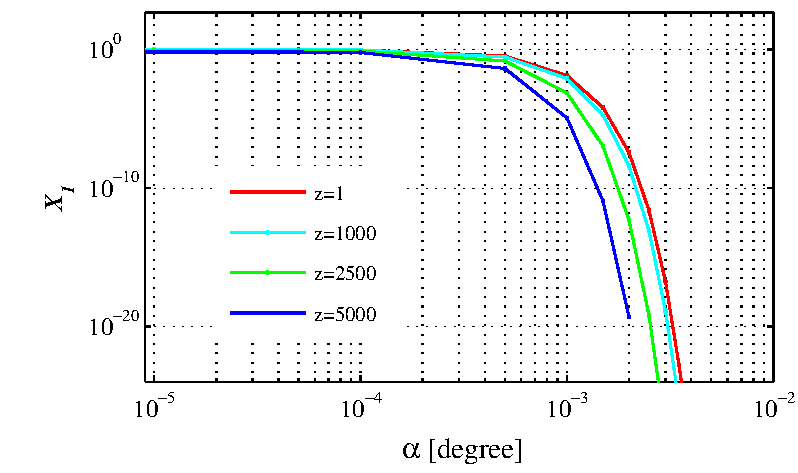
\includegraphics[scale =.7]{./Sec_Optics/scat-plot-1.pdf}
\caption{The coupling factor $X_1$ (direct back scattering) over the mirror angle
where the scattering process occurs.
The coupling factor rapidly goes to zero after $10^{-3}$ degrees.}
\label{fig:scat-plot-1}
\end{figure}

$\bullet$ Diagonal path scattering:
From the assumption using BRDF and the scattering angles
when the longer and the shorter path lengths of the rectangular cavity
are 10 km and 1 m respectively,
the amplitude of the small angle scatter is
$\eta (\phi _{\rm s})=3.8 \times 10^{-8}$,
of the large angle scatter is $\eta (\phi _{\rm s})=7.5 \times 10^{-6}$,
and of the small-and-short scatter is $\eta (\phi _{\rm SS})=4.1 \times 10^{-5}$.
%(coupling coefficient varies depending on the coupling point.)
Adding the coupling coefficients of all the possible paths
up to 5 incidents, the total coupling coefficient was calculated
to be $4.7 \times 10^{-11}$ when the intra cavity power is normalised as unity.
Therefore, one should be careful to consider the scattering field propagating
along the diagonal paths in the rectangular cavity.
In order to block the diagonal paths, placing baffles
inside the rectangular geometry will be useful
to prevent the scattered light coupling into the cavity mode.

%Taking the statistical sum of the eight scattered fields,
%the total amplitude of the scattered filed is $2.5 \times 10^{-12}$,
%while the laser power is normalised to be unity at each mirror.

$\bullet$ Gaussian tail effect:
The Gaussian tail effect is found to be negligible
with the optical parameters considered here.
In numerical simulations a length of 1 m for the shorter paths
in rectangular or bow-tie cavities was found to be sufficient
for the effect to be negligible.
%Although this length should be careful not be too close.


%\subsection{Summary}
Table~\ref{table:summary} shows a summary of the numerical evaluation.
The two-mirror cavity is the best configuration from the scattered-light
point of view because there are no spurious paths in the geometry.
For the other three configurations,
the direct back scattering and the Gaussian tail effect were found to be negligible.
One should be careful to consider the scattering field propagating
along the diagonal paths in the rectangular cavity.
If this geometry is to be used, the placement of baffles
inside the rectangular geometry will be necessary
to prevent the scattered light from propagating along the paths.



\begin{table}
\begin{center}
\begin{tabular}{|c|c|c|c|c|}
\hline
Type        & direct-back scattering &  Diagonal & Gauss. Tail \\ \hline
Two-mirror   &   N/A  &  N/A   & N/A   \\ \hline
Triangular     & $0$ &  N/A    & N/A   \\ \hline
Rectangular  &  $0$ &  $4.7\times 10^{-11}$ & 0\\ \hline
Bow-tie        &  $0$ &  N/A  & 0    \\ \hline
\end{tabular}
\caption{Summary of the scattering process for each geometry without
an amplification factor of the cavity.
The numbers are in amplitudes while the light power is normalised
to be unity inside the cavity.}
\label{table:summary}
\end{center}
\end{table}

